\chapter{Third-Party Code and Libraries}

If you have made use of any third party code or software libraries, i.e. any code that you have not designed and written yourself, then you must include this appendix. 

As has been said in lectures, it is acceptable and likely that you will make use of third-party code and software libraries. The key requirement is that we understand what is your original work and what work is based on that of other people. 

Therefore, you need to clearly state what you have used and where the original material can be found. Also, if you have made any changes to the original versions, you must explain what you have changed. 


\chapter{Class diagram}\label{ap_class}

\begin{figure}[H]
  \centering
  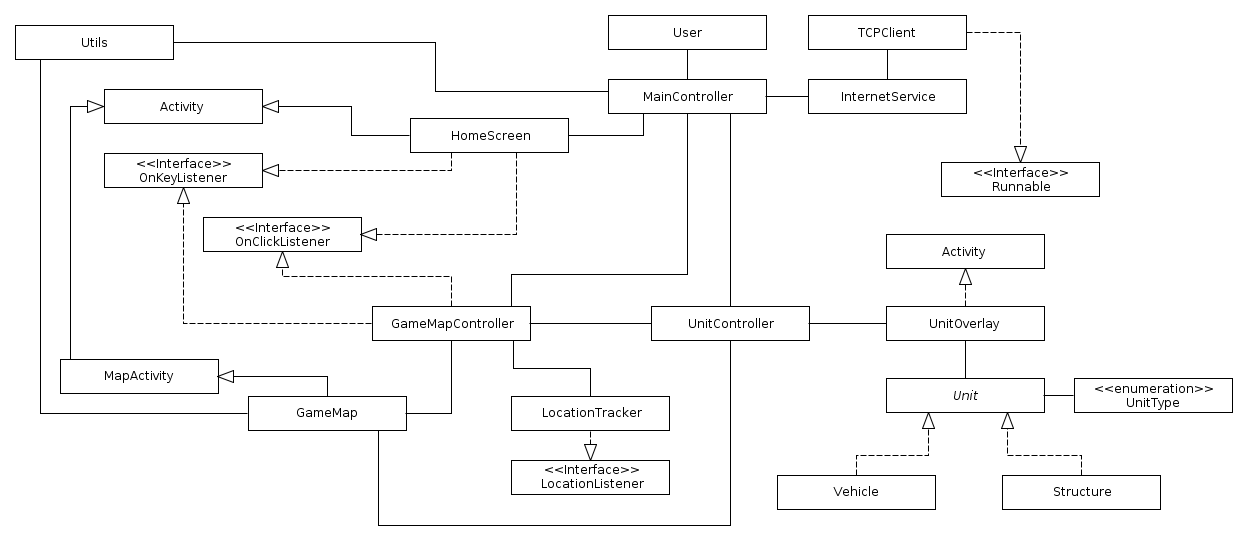
\includegraphics[height=0.3\textheight, angle=90]{Images/diagrams/class.png}
\end{figure}



\chapter{Server Testing - Message Generator}\label{server_testing}

\begin{verbatim}
#!/usr/bin/env python
import socket
import sys
import time
import re
import json


HOST = 'localhost'
PORT = 4565

sess = None
userID = None

try:
  sock = socket.socket(socket.AF_INET, socket.SOCK_STREAM)
  sock.connect((HOST, PORT))
except socket.error, msg:
  sys.stderr.write("[ERROR] %s\n" % msg[1])
  sys.exit(1)


while True:
  n = raw_input("> ")

  msgDic = dict()

  if n == "exit":
    break  # stops the loop
  else:
    match = re.findall("[^\s]+", n, re.M|re.I)
    if match:
      if match[0] == 'login':
        msgDic['action'] = "user.login"
        msgDic['user'] = match[1]
        msgDic['pass'] = match[2]
      elif match[0] == 'register':
        msgDic['action'] = "user.register"
        msgDic['user'] = match[1]
        msgDic['pass'] = match[2]
        msgDic['email'] = match[3]
      elif match[0] == 'location':
        msgDic['action'] = "user.location"

        if len(match) == 3:
          msgDic['lat'] = match[1]
          msgDic['lon'] = match[2]
        else:
          msgDic['lat'] = '52.35184333541474'
          msgDic['lon'] = '-1.966477632522583'
      elif match[0] == 'unit':
        msgDic['action'] = "unit.create"
        msgDic['type'] = match[1]
        msgDic['lat'] = match[2]
        msgDic['lon'] = match[3]
      elif match[0] == 'move':
        msgDic['action'] = "unit.move"
        msgDic['id'] = match[1]
        msgDic['lat'] = match[2]
        msgDic['lon'] = match[3]
      else:
        continue
      
      if sess:
        msgDic['sess'] = sess
      if userID:
        msgDic['userID'] = userID

      msg = json.dumps(msgDic)
      print '\x1b[38;5;15m' + "S " + msg + '\033[0m'
      sock.send(msg)


    else:
      continue


  rec = sock.recv(2048)
  try:
    data = json.loads(rec)

    #check for session data
    if data['action'] == 'user.login' and data['status'] == 1:
      sess = data['sess']
      #sess = 'cat'
      userID = data['userID']

    if data['status'] == 1:
      print '\x1b[38;5;46m' + "R " + rec + '\033[0m'
    else:
      print '\x1b[38;5;160m' + "R " + rec + '\033[0m'
  except ValueError:
    print rec


sock.close()

sys.exit(0)

\end{verbatim}